\chapter{Introduction}\label{chap:introduction}
% \section{Introduction}
% 2 pages
   \begin{figure}[!ht]
        \centering
        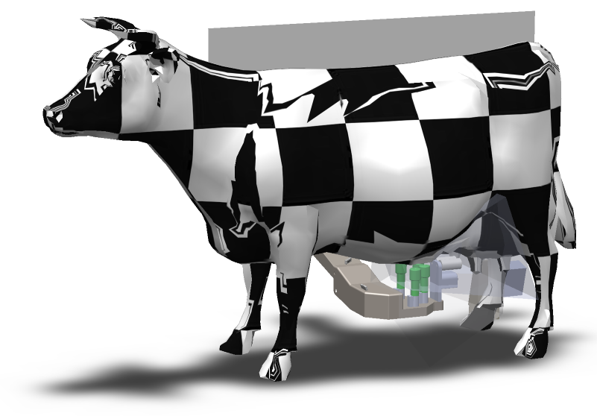
\includegraphics[width=0.7\textwidth]{images/cow_system.png}
        \caption{3D Prototype Model of the Cow Milking Robot}
        \label{fig:cow_fmc}
    \end{figure}
    
\section{Use Case: Improving the Cow Milking Automation}

\lipsum[2-5]

    % \begin{itemize}
    %     \item describe the general need for automated cow milking
    %     \item describe how the problem is currently being solved briefly
    
    %     \item describe the challenges in cow teat recognition: morphology/shapes and movement
    %     \item describe how these methods fail || describe challenges/limitations of current methods (sensors, etc, no memory)
    
    %     \item can solve this problem with computer vision briefly
    
    %     \item describe cow project main driver (The InIT's purpose) (do we mention how expensive current solutions are?)

    % \end{itemize}
\section{Towards 3D Object Detection}
\lipsum[2-5]

    % \begin{itemize}
    %     \item describe advancements in traditional computer vision for image interpretation
    %     \item list shortcomings/challenges we can overcome with computer vision
        
    %     \item describe advancements in computer vision with DL for object detection
    %     \item list shortcomings/challenges we can overcome with computer vision
        
    %     \item shortcoming1: no object permanence | objects out of sight
    %     \item shortcoming2: reliability of only detecting cow teats (?)
    %     \item HELP: shortcoming3: (?) (need to re-read the papers from gio)

    % \end{itemize}
\section{Problem Description}
\lipsum[2-3]
    \begin{itemize}
        \item in this work we answer the question: ---
        % \item we start by describing:
        %     \SubItem state of algorithms for cow milking
        %     \SubItem state of algorithms for 3d object detection
        %     \SubItem describe the system is able to localize cow teats in 3d space
        %     \SubItem describe the diverse algorithms we evaluated and tested (?)
        %     \SubItem finally we discuss the outcome of experiments and how to interpret conclusions
        %     \SubItem REWRITE/REUSE THIS SENTENCE FROM THESIS: We do not attempt to solve the specific use case of the ZHAW Summit XL Steel mobile robot, but aim to create an approach which is helpful in a large range of possible scenarios, similar to the way 3D mapping systems already enable robotic interaction today.
    \end{itemize}
